\subsection{Mutations and Guarantees}
\label{sec:granularityMutationInputs}
In the early stages of safety analysis on a complex critical system, it is beneficial to see what model elements may contribute to a property violation. While it is true that analysts will define faults based on their knowledge of the domain, at times in complex systems not all of these faults and their consequences are clear. Using the idea of mutations, we wish to see what the critical inputs to a system may be. 

As an example, we look once again at the sensor subsystem of a PWR as outlined in Chapter~\ref{chap:mcsGen}. Given a nominal system model containing the sensor subsystem and a single temperature sensor, we wish to see what model elements -- specifically guarantees -- are the \mustcov\  elements for the program. This tells the analyst that if these guarantees are violated, there are no paths to a proof of the property. 

To this end, we modified the equation remover implemented by Todorov, et al.~\cite{NFM2020Todorov} in JKind in order to collect killed guarantees from the program in Lustre. The results from the modified equation remover shows the following guarantees that are critical to any proof (Figure~\ref{}). 

After finding these results, we then defined a fault on the output governed by this guarantee and ran the minimal cut set generation on the fault model. As expected, this fault was in the minimal cut sets. While this example is sufficiently simple to illustrate the point, in complex models there can be multiple guarantees for a single component, many different components in a subsystem all of which are connected in various ways. It is obvious to anyone looking at the sensor subsystem model that this particular fault will violate the property. To this end, we turned our attention to a larger model: the Wheel Brake System as described in Section~\ref{chap:wbs}. At the time of this analysis, there were XX faults defined for XX components throughout the extended system model. The total number of contracts of the nominal model exceeded XXX. We ran this analysis to see if there were other faults that may have been overlooked during the development of the WBS model. 

A guarantee on the XX component was presented in the mutation analysis: \danielle{FIGURE OF GUARANTEE AND DESCRIPTION}. 

We defined a fault for the XX component as shown in Figure\danielle{make me}. Running minimal cut set generation with the additional constraint of one active fault, this fault is seen in the minimal cut sets; the violation of the property occurs when this fault is present. 

Performing a kind of mutation analysis could be beneficial during the fault modeling process to catch things that may be missed during the fault definition process. The initial foray into mutation testing results show that this has potential for integration into the safety annex. It was also clear that a better representation was needed for large models. In the case of the WBS mutation analysis, over XX guarantees were given as candidates for faults -- many of which already had faults associated with them. By integrating this feature into the fault analysis, these guarantees could be pruned from the output and save the user from pouring through potentially hundreds of guarantees. 

\subsection{Node Inputs and Mutation Testing}
The equation remover mutation also iterates through Lustre node inputs and performs the mutation one input at a time. The node inputs in the Lustre model correspond to the inputs and outputs of an AADL component as shown in Figure~\ref{fig:nodeInputsLustre}. 

\begin{figure}[h]
	\begin{center}
		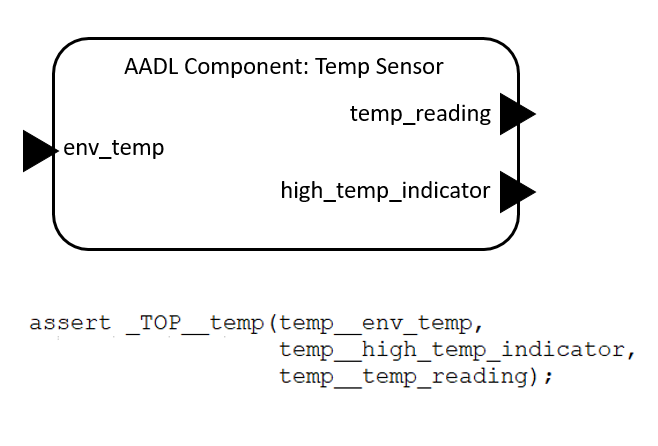
\includegraphics[scale=0.8]{images/nodeInputsLustre.PNG}
	\end{center}
	%\vspace{-1.5em}
	\caption{An AADL Component and Lustre Node Inputs}
	\label{fig:nodeInputsLustre}
\end{figure}

Given that the equation remover algorithm can perform this operation over node inputs, we can also gather information about critical outputs of components. Performing a similar extention to the equation remover algorithm, we collected all node input mutations that are killed and present them to the user. As an example, we show in Figure~\ref{fig:nodeInputsKilled} the analysis results on the nominal temperature subsystem example. 

\begin{figure}[h]
	\begin{center}
		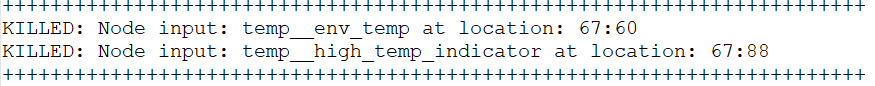
\includegraphics[scale=0.6]{images/nodeInputsKilled.PNG}
	\end{center}
	%\vspace{-1.5em}
	\caption{Temperature Node Inputs Killed by Equation Remover}
	\label{fig:nodeInputsKilled}
\end{figure}

Given that there exists an assumption on the temperature sensor input, we focus on the output. The only killed output was that of the high temperature indication, which tells us to prove the guarantee $\mathit{env\_temp} > 8 \iff \mathit{temp\_high}$, the output of this node is of utmost importance. Not surprisingly, when attaching a fault to this output, we get this fault in the minimal cut set for the top level property. 

As in the case with application of mutation testing on guarantees, node inputs also will require integration into the safety annex in order to filter out node inputs that have already been accounted for with faults in the extended system model. In large systems, this analysis is scalable and shows itself to be informative, but the outputs are unwieldy and large. Further work to rectify this would be required before use in large systems. 

The investigations into mutation testing applied to fault analysis were implemented in JKind and can be found at \url{https://github.com/dkstewart/jkind} on the {\em fault\_analysis\_mutations} branch.
